% 2010 年湖北卷理科第 15 题：以 AB 为直径的半圆，C 在 AB 上，DC⊥AB，CE⊥OD。
% 来源 PDF：普通高考/2010/2010湖北理.pdf，SHA-256 2cfb3d100d55f89c58fe4475caf29f039496afbd0f16d7a7d07857eed5759f55。
% 原页：第 1 页（A3 三栏）第 3 栏上部，书页码 597。
% 重绘依据：按 600 dpi 原页，A 在左、B 在右，O 为 AB 中点，C 在 O 与 B 之间（AC=a>b=CB）；
%   D 是过 C 的 AB 垂线与半圆的交点（D 在 C 正上方），连 AD、OD、BD；
%   E 为 C 到 OD 的垂足（OE≈OD/3），图中在 E、C 处有直角标记。
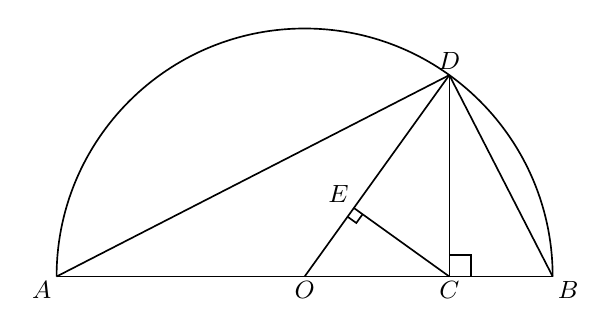
\begin{tikzpicture}[scale=1.05, semithick, every node/.style={inner sep=1.6pt, font=\small}]
  % 半圆与直径
  \draw (-3,0) -- (3,0);
  \draw (-3,0) arc (180:0:3);
  % 关键点
  \coordinate (A) at (-3,0);
  \coordinate (O) at (0,0);
  \coordinate (C) at (1.75,0);
  \coordinate (B) at (3,0);
  \coordinate (D) at (1.75,2.4360);
  \coordinate (E) at (0.5955,0.8291);
  % 连线
  \draw (A) -- (D);
  \draw (O) -- (D);
  \draw (B) -- (D);
  \draw (D) -- (C);
  \draw (C) -- (E);
  % C 处直角标记（DC 与 CB 之间）
  \draw (1.75,0.26) -- (2.01,0.26) -- (2.01,0);
  % E 处直角标记（EO 与 EC 之间）
  \draw (0.5197,0.7235) -- (0.6253,0.6477) -- (0.7011,0.7533);
  % 顶点与标注
  \node[below left]  at (A) {$A$};
  \node[below]       at (O) {$O$};
  \node[below]       at (C) {$C$};
  \node[below right] at (B) {$B$};
  \node[above]       at (D) {$D$};
  \node[above left]  at (E) {$E$};
\end{tikzpicture}
